\documentclass[withoutpreface,bwprint]{cumcmthesis} %去掉封面与编号页
\usepackage[framemethod=TikZ]{mdframed}
\usepackage{url}   % 网页链接
\usepackage{subcaption} % 子标题、
\usepackage{graphicx}
\title{“信息引航者”——基于MGCA的新闻推荐系统}
\usepackage{listings}
\lstset{language=Matlab}
\usepackage{pythonhighlight}
\usepackage{setspace}
\begin{document}
	
	\maketitle\thispagestyle{empty}
	\begin{abstract}
		信息技术不断发展,互联网上存在着大量信息,通过小红书、今日头条、bilibili等互联网平台获取信息是主要的信息获取途径之一。随着互联网上信息的越来越多,想要在海量信息中获取我们感兴趣或有需求的信息愈加困难。\par
		推荐系统的出现正是为了解决这种“信息过载”的问题。推荐系统已在互联网中得到了广泛的应用,并给应用它的企业带来了丰厚的利润。推荐系统给亚马逊带来了35\%的销售收入,给Netflix带来了高达75\%的消费,并且Youtube主页上60\%的浏览来自推荐服务。有关推荐系统的研究具有十分深远的意义与巨大的实用价值。\par
		
	\end{abstract}
	\setcounter{page}{1}
	\tableofcontents
	\newpage
	\section{引言}
	\subsection{研究背景及意义}
	\subsubsection{ 信息过载问题的解决迫在眉睫} 
	互联网高速发展,信息呈爆炸式增长,用户逐渐由信息匮乏时代迈入了信息过载时代——过量信息反而使得用户无法找到自己需要的信息。信息过载问题会产生一系列问题,比如用户体验变差、用户数量骤减、用户粘性降低等。
	信息爆炸的今天,个性化新闻推荐技术已经变成了许多新闻网站和App的关键技术。新闻的数据来源众多,可能一分钟就有成千上万条新的数据产生,在数据量激增的情况下,需要付出更多的人力成本,并且人工处理速度慢,效率十分低下。一套个性化新闻推荐系统刚好可以应用于有效缓解这种信息过载问题。如图1是新闻推荐系统通过个性化推荐实现精准化投放信息的流程示意。
	\begin{figure}[H]
		\centering
		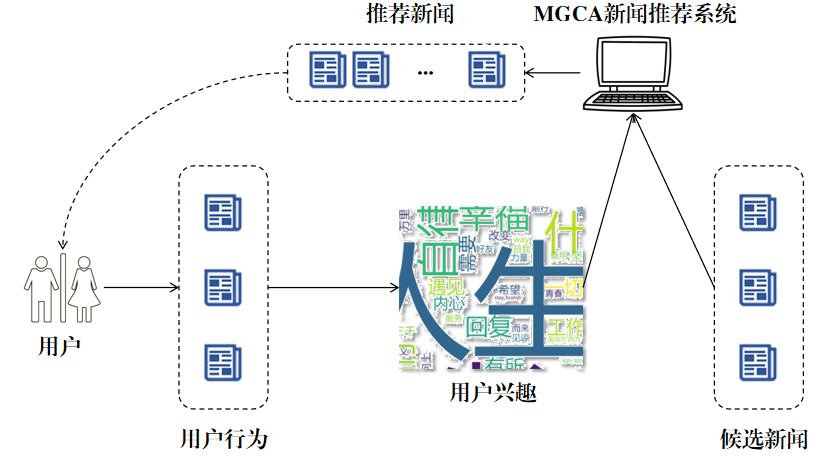
\includegraphics[width=0.95\textwidth]{2}
		\caption{个性化新闻推荐系统实现精准化投放信息}
		\label{fig:circuit-diagcam}
	\end{figure}
	\subsubsection{ 互联网与推荐系统的融合带来巨大的经济价值}
	目前互联网变现的主要方式均可以与推荐系统融合起来,创造巨大的经济价值,如图2展示了推荐系统与互联网融合时创造价值的几种常见途径:
	\begin{figure}[H]
		\centering
		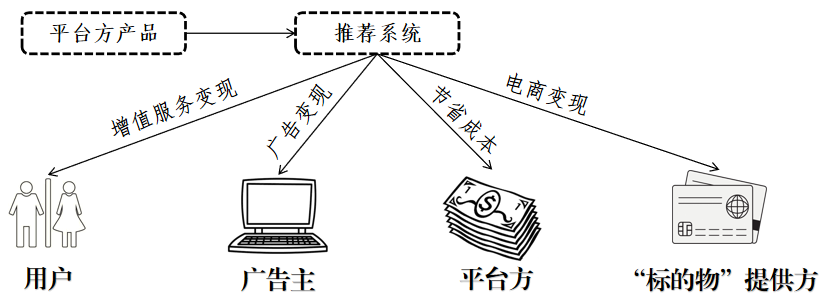
\includegraphics[width=0.95\textwidth]{1}
		\caption{推荐系统与互联网融合体现的经济价值}
		\label{fig:circuit-diagcam}
	\end{figure}
	$\bigstar$\textbf{增值服务变现:}增值服务主要是指基本服务以外的特色服务,如新闻平台常见的会员制。推荐系统通过精准把握用户兴趣,引导用户购买会员增值服务产品。推荐系统的个性化推荐服务不仅可以更加深层次的挖掘用户需求,还可以使更多相对冷门但优质的内容得到曝光与展示。\par
	$\bigstar$\textbf{广告变现:}用户方产品在互联网上投放广告,通过提高广告曝光以及用户点击广告获取权益。通过推荐系统的应用,可以在新闻APP中实现广告精准投放。广告业务偏轻公司一般都会选择流量外包方式做广告变现,通过新闻推荐系统提高广告精准投放率与用户点击率即是一种非常好的方式。\par
	$\bigstar$\textbf{节省成本变现:}推荐系统对平台方的贡献不仅在于直接的商业价值或是促进用户粘性、用户数量增长等,还可以用更少的成本实现最大程度的个性化新闻推荐,提高内容的分发效率。\par
	$\bigstar$\textbf{电商变现变现:}无论是传统意义的实体电商产品,还是网络小说、网络课程等虚拟电商产品,都可以通过提高分发商品效率,精准化投放促进商品售卖而提高商家分成,吸引商家入驻。总的来说,在电商变现方面,新闻推荐系统可以做到促进“标的物”提供方的生态逐步健全繁荣,获取更多经济效益。\par
	\subsubsection{ 响应国家发展和改革委员会“新基建”号召}
	 国家发改委于2020年4月首次明确了新型基础设施的范围包括以人工智能、云计算、区块链等为代表的新技术基础设施,新型基础设施建设对于打造经济新动能、重塑供应新链条、促进惠民新模式有重大意义,是当前稳经济、促增长的核心支撑。人工智能、云计算、物联网等现代信息科技依托新型基础设施建设得到了高速发展。\par
	 特别是处于疫情后时代,线下娱乐受到重创,线上娱乐成为青年群体最重要的娱乐方式之一。在当前的时代背景下,新闻推荐的研究有助于促进青年群体的幸福感,扩大新型基础设施建设的有效投资,有效对冲经济下行压力,有力支撑经济社会高质量恢复与持续发展。
	\subsection{相关研究现状}
	\subsubsection{ 推荐系统在工业界的应用现状}
	\subsubsection{ 推荐系统在学术界的研究现状}
	\subsection{项目架构总览}
	\subsubsection{ 项目整体框架}
	\subsubsection{ 项目优势与创新性}
	\newpage
	\section{模型技术路线及实现方案}
	\subsection{数据集选取}
	\subsubsection{ MIND数据集}
	\subsubsection{ glove词嵌入}
	\subsubsection{ 数据预处理}
	\subsection{方法介绍}
	\subsubsection{ 图神经网络}
	\subsubsection{ 注意力机制}
	\subsubsection{ Transformer}
	\subsubsection{ Fastformer}
	\subsection{模型架构}
	\subsubsection{ 总体架构}
	\subsubsection{ 候选新闻编码}
	\subsubsection{ 单词粒度感知候选新闻}
	\subsubsection{ 新闻粒度感知候选新闻}
	\subsubsection{ 实体粒度感知候选新闻}
	\subsection{模型评估}
	\subsubsection{ 与之前模型的性能对比}
	\subsubsection{ 消融实验}
	\newpage
	\section{软件工程与开发架构方案}
	\subsection{开发工具与框架}
	\subsection{新闻推荐系统软件落地示例}
	\subsubsection{ 软件周期模型}
	\subsubsection{ 软件开发模型}
	\subsubsection{ 数据库设计}
	\subsubsection{ UML设计}
	\subsubsection{ 软件功能演示}
	\subsubsection{ 兼容性测试与稳定性测试}
	$\bigstar$可执行测试:分别部署到不同性能的电脑上运行测试,均成功运行,网页反馈
	均在35ms到45ms左右,不存在延迟和卡顿现象,该系统对电脑的配置要求较低。\par
	$\bigstar$功能测试:所有功能均可正常运行使用,可视化动态大屏显示正常,首页展示
	效果正常,查询功能正常,链接页面跳转正常。\par
	$\bigstar$兼容测试:在 Windows、Linux、Mac等操作系统可以正常访问。谷歌浏览器、
	火狐浏览器、QQ 浏览器、360 浏览器等运行均正常。Windows操作系统的python版
	本为3.6以上、tensorflow2.14.0 版本环境可以正常运行平台。\par
	$\bigstar$安全测试:本项目采取的是 https 协议,安全性和可靠性比较高,jupyter 环境
	提供了三种安全级服务配置,可以按照实际的需求提升安全等级。\par
	\newpage
	\section{商业模式构建与经营管理}
	\subsection{市场竞争分析}
	\subsection{投资回报分析}
	\subsection{盈利方式}
	\subsubsection{ 提供整套低耦合工业界解决方案}
	\subsubsection{ 提供整套成熟软件系统}
	\subsection{财务管理}
	\subsection{营销战略}
	\newpage
	
	%参考文献
	\begin{thebibliography}{9}%宽度9
		[1]陈昌凤,袁雨晴.智能新闻业:生成式人工智能成为基础设施[J].内蒙古社会科学,2024,45(01):40-48.DOI:10.14137/j.cnki.issn1003-5281.2024.01.006.
	\end{thebibliography}
	
	\newpage
\end{document}
